\documentclass{beamer}
\mode<presentation>
{
  \usetheme{Madrid}     
  \usecolortheme{default} 
  \usefonttheme{serif} 
  \setbeamertemplate{navigation symbols}{}
  \setbeamertemplate{caption}[numbered]
} 

\usepackage{xcolor}
\usepackage{mathtools}   
%\usepackage[english]{babel}
%\usepackage{Times}
%\usepackage{tgpagella}
\usepackage[utf8x]{inputenc}    %%helps with some symbols
\usepackage{amsmath}            %%math symbols
\usepackage{amssymb}
\usepackage{amsfonts} 
\usepackage{multirow}
\setlength{\marginparwidth}{2cm}
\usepackage{todonotes}
\usepackage{listings}
\lstset{basicstyle=\ttfamily}
\usepackage{comment}
\usepackage{tikz}
\usepackage{tikz-cd}

\usepackage{mathabx}
\usepackage[percent]{overpic}
% Source - https://tex.stackexchange.com/a/119985
% Posted by latex user, modified by community. See post 'Timeline' for change history
% Retrieved 2026-03-26, License - CC BY-SA 4.0

\usepackage{graphicx}           %%helps with images
\usepackage[export]{adjustbox}  %%helps with algning images
\usepackage{subcaption}         %%subfigures
\usepackage{mathrsfs}
\def\insertauthorindicator{}
\def\insertinstituteindicator{}

% LaTeX

% ConTeXt
%\setupbodyfont[modern]


%\usepackage{tgheros}

\title[Dietmaier Optimization]{Dietmaier Optimization and Omnitropic descent}
\subtitle{}
\author[Deepak M S]{Deepak M S\\ \vspace{2mm}(Joint work with Taylor Brysiewicz, David K. Johnson)}
\institute[Western]{University of Western Ontario}
\vspace{4mm}
\date{\small{AMS Spring Southeastern Sectional\\
Savannah, GA}}

\newcommand{\cat}{\mathrm{cat}}
\newcommand{\dime}{\mathrm{dim}}
\newcommand{\TC}{\mathrm{TC}}
\newcommand{\secat}{\mathrm{secat}}
\newcommand{\zcl}{\mathrm{zcl}}
\newcommand{\Q}{\mathbb{Q}}
\newcommand{\C}{\mathbb{C}}
\newcommand{\R}{\mathbb{R}}
\newcommand{\F}{$\mathcal{F}$}

%\AtBeginSection[]
%{
  %\begin{frame}
    %\frametitle{Table of Contents}
    %\tableofcontents[currentsection]
  %\end{frame}
%}

\begin{document}
\begin{frame}
  \titlepage
\end{frame}

\begin{comment}
\begin{frame}{Table of contents}
\frametitle{}
\tableofcontents  
\end{frame}
\end{comment}

\section{Introduction}% 

\begin{comment}

\begin{frame}{Parametrized polynomial systems}
	\textbf{Notation:}\\
	Suppose $F({\color{blue}z},{\color{red}p}) = (f_1, \cdots, f_n)$ is a square parametrized polyomial system.
	
	%\centering
	Here, {\color{red}$p = (p_1,\cdots,p_k)$} : parameters,
	{\color{blue}$z= (z_1,\cdots,z_n)$} : variables. \pause
	
	\vspace{4mm}
	\textbf{Example:}
	\[
	F({\color{blue}z},{\color{red}p}) = 
\begin{bmatrix}
	{\color{red}w_1} {\color{black}-} \frac{\color{black}1}{\color{black}3} {\color{black}(} {\color{blue}s_1} {\color{black}+} {\color{blue}s_1 c_2} {\color{black}-} {\color{blue}s_2 c_1} {\color{black})} &{\color{black}} \\
	{\color{blue}c_1}^{\color{black}2} {\color{black}+} {\color{blue}s_1}^{\color{black}2} {\color{black}- 1} &{\color{black}} \\
	{\color{red}w_2} {\color{black}-} \frac{\color{black}1}{\color{black}3} {\color{black}(} {\color{blue}s_2} {\color{black}+} {\color{blue}s_2 c_1} {\color{black}-} {\color{blue}s_1 c_2} {\color{black})} &{\color{black}} \\
	{\color{blue}c_2}^{\color{black}2} {\color{black}+} {\color{blue}s_2}^{\color{black}2} {\color{black}- 1} &{\color{black}}
\end{bmatrix}
\]
\end{frame}
\end{comment}


\begin{frame}[fragile]{Setting and goal}
 %Add the Kuramot Model picture along with the equation.
 \[\mathcal{F}(z, p)= \begin{bmatrix}
 	f_1 \\ \vdots\\ f_n
 \end{bmatrix} \subseteq \C[p_1,\cdots, p_k][x_1,\cdots,x_n]\]
%\begin{comment}
\begin{figure}
      \begin{overpic}[width=0.65\textwidth, tics=10]{figs/KuramotoModel_proj5.pdf}
      	\put (33,39) {\tiny $y_1$}
      	\put (33,42) {\tiny $\widebar{y_1}$}
      	\put (33,45) {\tiny $y_2$}
      	\put (33,48) {\tiny $\widebar{y_2}$}
      	\put (33,53) {\tiny $x_1$}
      	\put (33,56) {\tiny $x_2$}
      	\put (33,15) {\tiny $p$}
      	\put (67,56) {$V(\mathcal{F})$}
      	\put (70,44) {$\Bigg\downarrow$}
      	\put (68,45) {\tiny $\pi$}
      	\put (73,45) {\tiny $6$-to-$1$}
      \end{overpic}
      \caption*{ \textbf{Goal} : To find as many real solutions as possible.}
       % \label{fig:my_label}
 \end{figure}
   
  
%\end{comment}
% Source - https://tex.stackexchange.com/a/20802
% Posted by Martin H, modified by community. See post 'Timeline' for change history
% Retrieved 2026-03-28, License - CC BY-SA 3.0


	

 %Twentyseven lines on a conic:
 
%Consider if Twenty Seven Lines is a better example.
 \end{frame}
 

% \begin{frame}
% The system is given by the polynomial equations
% \[{\color{blue}\omega_i} -\frac{1}{N}\sum_{j = 1}^n(s_ic_j-c_js_i) = 0\] 
% and 
% \[s_i^2 +c_i^2 - 1 = 0\]
% where $i$ ranges from $i$ to $N$.
% The $\omega_i$s are the parameters of the polynomial system whereas $s_i$s and $c_j$s constitute the variables.
% \end{frame}
\section{Hill-climbing}

\begin{comment}
\begin{frame}{Hill-climbing}
$<$ Explain Hill Climbing, maybe add a picture$>$.

\end{frame}
\end{comment}

\begin{frame}{Dietmaier's idea}
\begin{figure}
        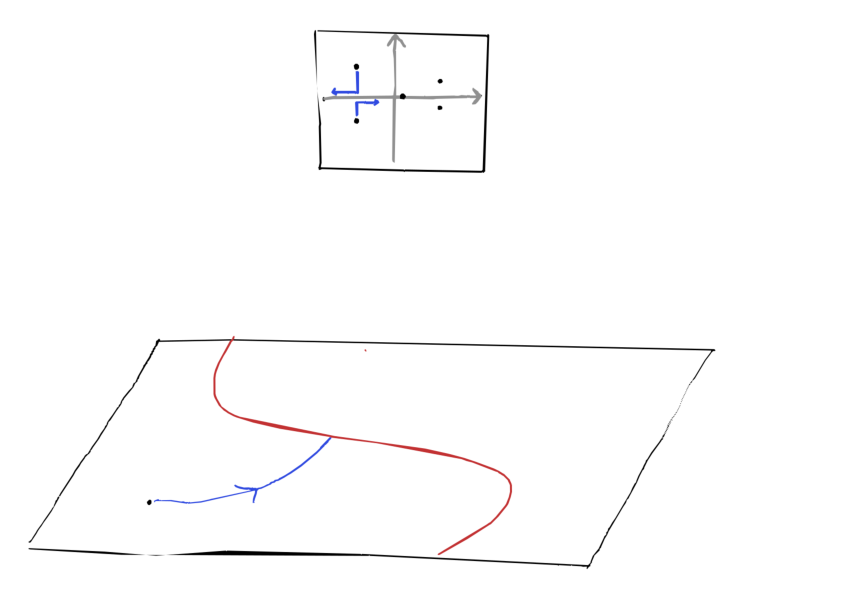
\includegraphics[scale=0.5]{figs/slide_2_img1.pdf}
       \caption*{Dietmaier's idea: Move in $\R_p^k$ to smash conjugate solutions together. To do this, we need to minimize $||\text{imag } y_i (p)||$.}
       % \label{fig:my_label}
\end{figure}
    
%We try to minimise $ {\color{violet}\mathcal{D}(p) =\min\{||\text{Im}(z)||\,:\,z \text{ is not real}, F(z, p) = 0\}}$ while also ensuring that the {\color{blue}number of real solutions} never goes down.
\end{frame}


\begin{comment}
\begin{frame}%{Versatile Optimization}
\begin{figure}
\begin{minipage}{0.45\textwidth}
	\centering
	\includegraphics[scale=0.3]{KuramotoModel_taboo.pdf}
	\caption{\lstinline|\#real_solutions|}
\end{minipage}\hfill
\begin{minipage}{0.45\textwidth}
	\centering
	\includegraphics[scale=0.3]{KuramotoModel_objective.pdf}
	\caption{Dietmaier}
\end{minipage}       
       % \label{fig:my_label}
    \end{figure}
\end{frame}

\begin{frame}%{Versatile Optimization}
\begin{figure}
\begin{minipage}{0.45\textwidth}
	\centering
	
\includegraphics[scale=0.3]{dietmaier_taboo.pdf}
	\caption{\lstinline|\#real_solutions|}
\end{minipage}\hfill
\begin{minipage}{0.45\textwidth}
	\centering
	
\includegraphics[scale=0.3]{dietmaier_scheme.pdf}
	\caption{dietmaier}
\end{minipage}       
       % \label{fig:my_label}
    \end{figure}
\end{frame}


\begin{frame}{Hill-climbing}
\begin{figure}
        
\includegraphics[scale=0.55]{Hill-Climbing.png}
      % \caption{For complex solutions to turn real, two conjugate solutions must merge.}
       % \label{fig:my_label}
\end{figure}
\end{frame}
\\

\begin{frame}{Versatile Optimization}
Talk about taboo function and objective function
\end{frame}

\begin{frame}{Some strategies for hill-climbing} 
\textbf{Raincloud}

\begin{figure}
	
\includegraphics[scale=0.55]{Kuramotoraincloud.pdf}
	 \caption{Without raincloud updates.}
	% \label{fig:my_label}
\end{figure}
\end{frame}

\begin{frame}{Some strategies for hill-climbing} 
	\begin{figure}
		
\includegraphics[scale=0.55]{after_raincloud.pdf}
		\caption{After raincloud updates.}
		% \label{fig:my_label}
	\end{figure}
\end{frame}
\begin{frame}{Some strategies for hill-climbing}
	\textbf{Ellipsoidal sampling}
	% Source - https://tex.stackexchange.com/a/119985
	% Posted by latex user, modified by community. See post 'Timeline' for change history
	% Retrieved 2026-03-26, License - CC BY-SA 4.0
	
	\begin{figure}[t!]
		\centering
		\begin{subfigure}[t]{0.5\textwidth}
			\centering
			
\includegraphics[height=1.75in]{hallway_uniform_sampling.png}
			\caption{Usual uniform sampling}
		\end{subfigure}%
		~ 
		\begin{subfigure}[t]{0.5\textwidth}
			\centering
			
\includegraphics[height=1.75in]{hallway_ellipsoid_sampling.png}
			\caption{Ellipsoidal sampling}
		\end{subfigure}
		\caption*{}
	\end{figure}
\end{frame}
\end{comment}

%\section{Gradient Descent}%Why versatile? and How versatile? maybe




%\begin{frame}%{Versatile Optimization}
%\begin{figure}
%        \includegraphics[scale=0.5]%{dietmaier_scheme.pdf}
%       \caption{Dietmaier Objective Score on a cross-section of parameter space of TwentySevenLines enumerative problem.}
       % \label{fig:my_label}
%    \end{figure}
%\end{frame}

\begin{frame}{Dietmaier's choice}
Choice: Follow gradient of $||\text{imag } y_i (p)||$ with respect to $p$, for $y_i$ with the \textbf{smallest} imaginary part.\\
Demand: No real solutions are lost in the process.
\begin{figure}
	\begin{overpic}[width=0.8\textwidth, tics=10]{figs/dietmaiers_choice_not_ideal_2.pdf}
	\put (11,4) {\tiny $2$}
	%\put (15,4) {\tiny $4$}
	\put (22,4) {\tiny $6$}
	\put (30.5,4) {\tiny $4$}
	\put (37,4) {\tiny $2$}
	\put (48.5,4) {\tiny $0$}
	\put (59.5,4) {\tiny $2$}
	\put (70.5,4) {\tiny $4$}
	\put (15.0,4) {\tiny $4$}
	\put (84.5,4) {\tiny $2$}
	%\put (70.0,0.8) {$\longleftarrow$}
	\end{overpic}
	\caption{ The demand that no real solutions are lost, will prevent us from reaching the chamber with $6$ solutions.}
	% \label{fig:my_label}
\end{figure}
\end{frame}

\begin{frame}%{Dietmaier's choice}
	\begin{figure}
		\begin{overpic}[width=0.7 \textwidth, tics=10]{figs/kuramoto_dietmaier.pdf}
			
			%\put (70.0,0.8) {$\longleftarrow$}
		\end{overpic}
		% \label{fig:my_label}
	\end{figure}
\end{frame}


\begin{frame}%{Dietmaier's choice}
	\begin{figure}[t!]
		\centering
		\begin{subfigure}[t]{0.5\textwidth}
			\centering
			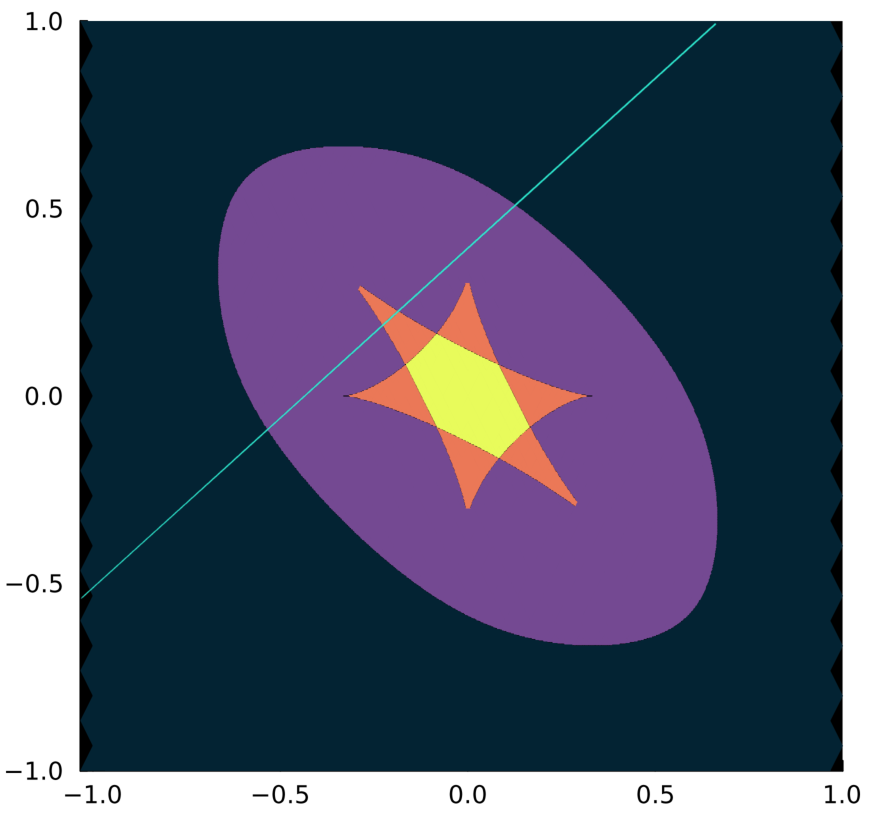
\includegraphics[height=1.75in]{figs/KuramotoModel_restriction_2.pdf}
			\caption{Kuramoto model, restricted}
		\end{subfigure}%
		~ 
		\begin{subfigure}[t]{0.5\textwidth}
			\centering
			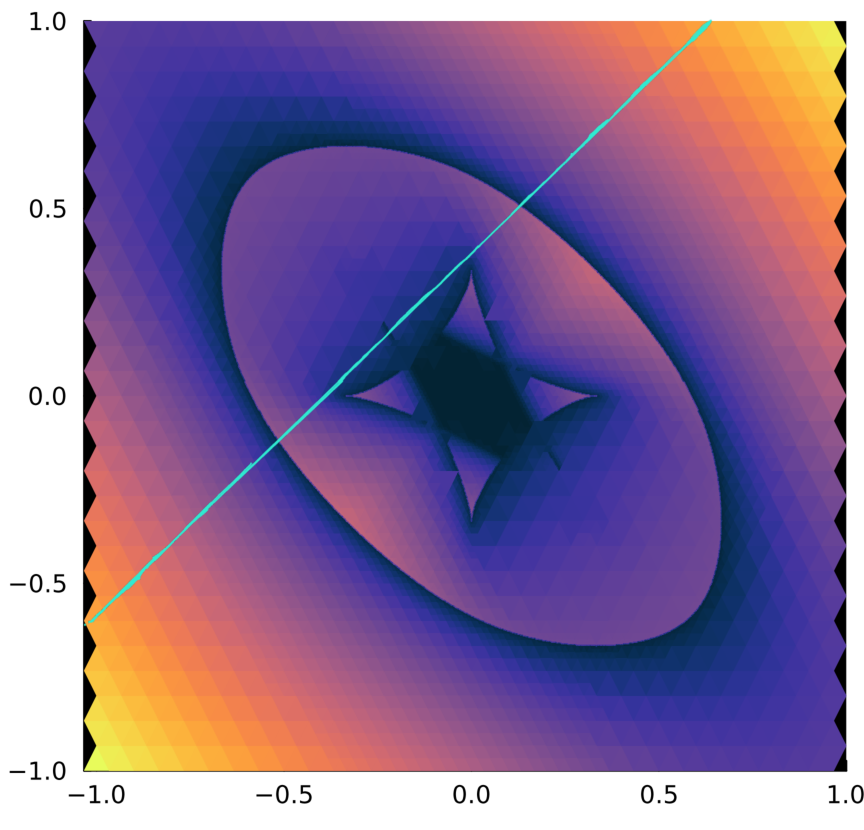
\includegraphics[height=1.75in]{figs/KuramotoModel_restriction_objective_2.pdf}
			\caption{The dietmaier function value}
		\end{subfigure}
		\caption*{}
	\end{figure}
\end{frame}


\begin{comment}

\begin{frame}{Gradient vector field}
\begin{figure}
	        
\includegraphics[scale=0.5]{kuramotomodel_gradient_field.png}
	%       \caption{Dietmaier Objective Score on a cross-section of parameter space of TwentySevenLines enumerative problem.}
	% \label{fig:my_label}
\end{figure}
\end{frame}


\section{Implementation}

\begin{frame}{Implementation}
We note that we do not need to specifically work with the {\color{violet}Dietmaier's objective function}.
Our implementation leverages the inherent flexibility within each chamber. Rather than strictly following the gradient of the minimal imaginary component  ${\color{violet}\min \{ ||\text{Im} (z)||\}}$, we will consider the vectors
\[v_i= \nabla\big(||\text{Im}(z)||\big)\bigg|_{(z_i,p)}\] when $z_i$ non-real. This allows us to strategically select and follow any of the directed flows..
\end{frame}




\begin{frame}{Omnitropic and lazy}
	
\end{frame}
\begin{frame}{Interesting examples}
\begin{itemize}
\item \textbf{Finding a generic quintic 3 fold for which the number of real lines on it is the maximum}:\\ 
\vspace{4mm}
In the enumerative problem of finding a generic quintic 3 fold for which the number of real lines on it is the maximum, we have:\\ \pause 
\vspace{4mm}
\begin{itemize}
	\item Upper bound: 2875 (the generic number of the complex solutions)
	\item Lower bound : atleast 15.

\end{itemize}\pause

\vspace{4mm}
\centering
 The maximum number of real solutions we found:  203.

\end{itemize}
\end{frame}

\end{comment}

\begin{frame}{Flow directions}
	\begin{figure}
		\begin{overpic}[width=0.7\textwidth, tics=10]{figs/KuramotoModel_vis.pdf}
			\put (40,25) {\tiny $v_1$}
			\put (42,28) {\tiny $\gamma_1$}
			\put (34,28) {\tiny $v_2$}
			\put (37,32) {\tiny $\gamma_2$}
		\end{overpic}
		% \label{fig:my_label}
	\end{figure}
	\begin{align*}
		v_1 &= -\nabla_p || \text{imag} (y_1(p))||& \gamma_1 &= \text{path that takes the direction $v_1(p)$ at $p$}\\
		v_2 &= -\nabla_p || \text{imag} (y_2(p))|| & \gamma_2 &= \text{path that takes the direction $v_2(p)$ at $p$.}
	\end{align*}
\end{frame}

\begin{frame}
	\begin{figure}
		\begin{overpic}[width=0.7\textwidth, tics=10]{figs/KuramotoModel_vis.pdf}
			\put (40,25) {\tiny $v_1$}
			\put (42,28) {\tiny $\gamma_1$}
			\put (34,28) {\tiny $v_2$}
			\put (37,32) {\tiny $\gamma_2$}
		\end{overpic}
		% \label{fig:my_label}
	\end{figure}
	\textbf{Lazy}: These flows can be travelled by tracking one path, and not $d$ paths at once. Flow tracking is very fast!\\
	\textbf{Observation}: These flows need not end up in a neighbouring chamber. They might travel over the discriminant.
\end{frame}
\begin{frame}[fragile]{Omnitropic descent}
	% https://q.uiver.app/#q=WzAsMTMsWzMsMCwicF8xIl0sWzEsMiwicV8xIl0sWzUsMiwicV9rIl0sWzIsMiwicV8yIl0sWzAsNCwiXFxidWxsZXQiXSxbMSw0LCJcXGJ1bGxldCJdLFsyLDQsIlxcYnVsbGV0Il0sWzUsNCwiXFxidWxsZXQiXSxbNiw0LCJcXGJ1bGxldCJdLFszLDIsIlxcY2RvdHMiXSxbMyw0LCJcXGNkb3RzIl0sWzQsMiwiXFxjZG90cyJdLFs0LDQsIlxcY2RvdHMiXSxbMCwxXSxbMCwzXSxbMSw0XSxbMSw1XSxbMyw2XSxbMiw3XSxbMiw4XSxbMCwyXV0=
	\[\begin{tikzcd}
		&&& {p_1} &&& \\
		\\
		& {q_1} & {q_2} & \cdots & \cdots & {q_k} \\
		\\
		r_1 & r_2 & r_3 & \cdots & \cdots & r_{s-1} & r_s 
		\arrow[from=1-4, to=3-2]
		\arrow[from=1-4, to=3-3]
		\arrow[from=1-4, to=3-6]
		\arrow[from=3-2, to=5-1]
		\arrow[from=3-2, to=5-2]
		\arrow[from=3-3, to=5-3]
		\arrow[from=3-6, to=5-6]
		\arrow[from=3-6, to=5-7]
	\end{tikzcd}\]
	\textbf{Dietmaier}: Chooses a branch of $y(p)$ at each step.\\
	\textbf{Omnitropic}: Follow the directions given by each of the $y_i$s lazily, and then solves for the fibres and then repeats on $q_i$s with the most number of real solutions.
\end{frame}

\begin{frame}%{Example}
	\begin{figure}
		\begin{overpic}[width=0.7\textwidth, tics=10]{figs/flow_Example.pdf}
		\end{overpic}
		% \label{fig:my_label}
	\end{figure}
\end{frame}

\begin{frame} 
	\begin{center} 
		
			% \color{blue}
		
\hspace{5mm}
\Huge Thank You!
\end{center}
\end{frame}
\end{document}               